%% ------------------------------------------------------------------------- %%
\chapter{Introdução}
\label{cap:introducao}

Com o avanço na tecnologia da computação, novos softwares são criados para
suprir necessidades de diversos domínios. Atualmente, o ecossistema de software
é bem diversa: Sistemas web desenvolvidos codificados em Ruby, Python, Java; até
sistemas operacionais, destinados a controlar os recursos do hardware, escritos
em C.

Independente da razão pela qual o software foi desenvolvido, em algum ponto o
código da aplicação será transformado em linguagem de máquina por um
compilador, mesmo que ele seja executado por um interpretador. Um compilador
nada mais é que um software que traduz um código em uma linguagem de
programação $A$ para outra linguagem $B$ \citep{dragonbook}.

Compiladores são programas largamente adotados pela indústria e academia. Muito
esforço e pesquisa foi e ainda é empregado para que eles produzam código
correto e rápido. Existem projetos enormes destinados a desenvolver e
aprimorá-los, como o Gnu Compiler Collection, capaz de traduzir diversas
linguagens como C, C++ e Fortran, para linguagem de máquina. Há também outros
projetos menores como o F2C, um compilador de Fortran para C, utilizado em
ambientes onde não há um compilador Fortran disponível.  Embora ainda seja
possível escrever código em linguagem de máquina, o que tornaria um compilador
desnecessário, isto é uma prática extremamente incomum nos projetos
contemporâneos a este trabalho
\citep{githuboctoverse} (vide Figura \ref{fig:github_2017}).

\begin{figure}[ht]
 \centering
 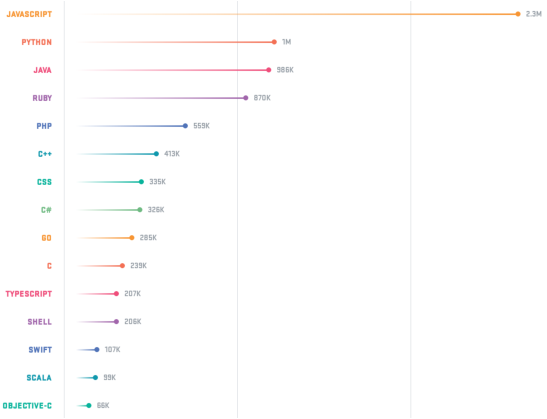
\includegraphics[scale=1.0]{github_2017.pdf}
 \caption{As 15 linugagens mais usadas em 2017. Fonte: \cite{githuboctoverse}}
 \label{fig:github_2017}
\end{figure}

Grandes projetos podem conter milhões de linhas de código, e até mesmo
construir novas linguagens para facilitar o desenvolvimento de novas
funcionalidades. Por exemplo, O GCC contém uma linguagem própria para facilitar
a adição de novas otimizações para gerar código mais rápido, que em seguida é
compilado em um único arquivo C, para (1) aproveitar as otimizações já
implementadas do próprio compilador C, e (2) evitar reescrever várias
funcionalidades já implementadas no compilador. Infelizmente, este processo
gera um gargalo na compilação do projeto em máquinas manycore, pois o GCC não é
capaz de compilar um arquivo em paralelo, e todo o paralelismo na fase de
compilação é providenciado pelo GNU Make, que apenas fornece uma granularidade
a nível dos arquivos. Tal problema pode parecer uma característica peculiar do
projeto GCC, entretanto discussões na lista de email do GCC \citep{mailgcc} e Phoronix levaram
usuários a relatar o mesmo problema em seus projetos, algo que um compilador
que seja capaz de compilar um único arquivo em paralelo é capaz de mitigar.
Outra possível solução para cada projeto é quebrar o arquivo em outros
arquivos, e utilizar o esquema de paralelismo do GNU Make, mas isto implica em
uma modificação na estrutura do projeto, o que pode não ser o ideal.

Por fim, atualmente existe uma tendência para que os processadores sejam cada vez mais
paralelos. Ambas a AMD e Intel oferecem produtos com até 16 núcleos para
entusiastas, e é possível encontrar servidores com mais de 64 núcleos
disponíveis para processamento. Compiladores que compilam em paralelo poderiam
aproveitar esse recurso, pois diminuiria o tempo de compilação de um projeto,
ou até mesmo uma suíte de testes que necessita recompilação antes de sua
execução.

É perfeitamente compreensível que pouca pesquisa seja realizada a
respeito de paralelização de compiladores. Compiladores se apoiam algoritmos em
grafos e analisadores léxicos-sintáticos, que geralmente são difíceis de
paralelizar no caso geral. É necessário um caso extremo -- um arquivo muito
grande -- para que haja algum benefício de paralelização; e este caso existe
dentro do próprio projeto do GCC, conforme discutido acima.



%Escrever bem é uma arte que exige muita técnica e dedicação e,
%consequentemente, há vários bons livros sobre como escrever uma boa
%dissertação ou tese. Um dos trabalhos pioneiros e mais conhecidos nesse
%sentido é o livro de
%%Umberto Eco~\cite{eco:09} % usando o estilo alpha
%Umberto~\citet{eco:09} % usando o estilo plainnat
%intitulado \emph{Como se faz uma tese}; é uma leitura bem interessante mas,
%como foi escrito em 1977 e é voltado para trabalhos de graduação na Itália,
%não se aplica tanto a nós.
%
%Sobre a escrita acadêmica em geral, John Carlis disponibilizou um texto curto
%e interessante~\citep{carlis:09} em que advoga a preparação de um único
%rascunho da tese antes da versão final. Mais importante que isso, no
%entanto, são os vários \textit{insights} dele sobre a escrita acadêmica.
%Dois outros bons livros sobre o tema são \emph{The Craft of Research}~\citep{craftresearch}
%e \emph{The Dissertation Journey}~\citep{dissertjourney}. Além disso, a USP
%tem uma compilação de normas relativas à produção de documentos
%acadêmicos~\citep{usp:guidelines} que pode ser utilizada como referência.
%
%Para a escrita de textos especificamente sobre Ciência da Computação, o
%livro de Justin Zobel, \emph{Writing for Computer Science}~\citep{zobel:04}
%é uma leitura obrigatória. O livro \emph{Metodologia de Pesquisa para
%Ciência da Computação} de
%%Raul Sidnei Wazlawick~\cite{waz:09} % usando o estilo alpha
%Raul Sidnei~\citet{waz:09} % usando o estilo plainnat
%também merece uma boa lida. Já para a área de Matemática, dois livros
%recomendados são o de Nicholas Higham, \emph{Handbook of Writing for
%Mathematical Sciences}~\citep{Higham:98} e o do criador do \TeX{}, Donald
%Knuth, juntamente com Tracy Larrabee e Paul Roberts, \emph{Mathematical
%Writing}~\citep{Knuth:96}.
%
%Apresentar os resultados de forma simples, clara e completa é uma tarefa que
%requer inspiração. Nesse sentido, o livro de
%%Edward Tufte~\cite{tufte01:visualDisplay}, % usando o estilo alpha
%Edward~\citet{tufte01:visualDisplay}, % usando o estilo plainnat
%\emph{The Visual Display of Quantitative Information}, serve de ajuda na
%criação de figuras que permitam entender e interpretar dados/resultados de forma
%eficiente.
%
%Além desse material, também vale muito a pena a leitura do trabalho de
%%Uri Alon \cite{alon09:how}, % usando o estilo alpha
%Uri \citet{alon09:how}, % usando o estilo plainnat
%no qual apresenta-se uma reflexão sobre a utilização da Lei de Pareto para
%tentar definir/escolher problemas para as diferentes fases da vida acadêmica.
%A direção dos novos passos para a continuidade da vida acadêmica deveria ser
%discutida com seu orientador.
%
%%% ------------------------------------------------------------------------- %%
%\section{Considerações de Estilo}
%\label{sec:consideracoes_preliminares}
%
%Normalmente, as citações não devem fazer parte da estrutura sintática da
%frase\footnote{E não se deve abusar das notas de rodapé.\index{Notas de rodapé}}.
%No entanto, usando referências em algum estilo autor-data (como o estilo
%plainnat do \LaTeX{}), é comum que o nome do autor faça parte da frase. Nesses
%casos, pode valer a pena mudar o formato da citação para não repetir o nome do
%autor; no \LaTeX{}, isso pode ser feito usando os comandos
%\textsf{\textbackslash{}citet}, \textsf{\textbackslash{}citep},
%\textsf{\textbackslash{}citeyear} etc. documentados no pacote
%natbib \citep{natbib}\index{natbib} (esses comandos são compatíveis com biblatex
%usando a opção \textsf{natbib=true}, ativada por padrão neste modelo). Em geral,
%portanto, as citações devem seguir estes exemplos:
%
%\small
%\begin{verbatim}
%Modos de citação:
%indesejável: [AF83] introduziu o algoritmo ótimo.
%indesejável: (Andrew e Foster, 1983) introduziram o algoritmo ótimo.
%certo: Andrew e Foster introduziram o algoritmo ótimo [AF83].
%certo: Andrew e Foster introduziram o algoritmo ótimo (Andrew e Foster, 1983).
%certo (\citet ou \citeyear): Andrew e Foster (1983) introduziram o algoritmo ótimo.
%\end{verbatim}
%\normalsize
%
%O uso desnecessário de termos em língua estrangeira deve ser evitado. No entanto,
%quando isso for necessário, os termos devem aparecer \textit{em itálico}.
%\index{Língua estrangeira}
%% index permite acrescentar um item no indice remissivo
%
%Uma prática recomendável na escrita de textos é descrever as
%legendas\index{Legendas} das figuras e tabelas em forma auto-contida: as
%legendas devem ser razoavelmente completas, de modo que o leitor possa entender
%a figura sem ler o texto onde a figura ou tabela é citada.\index{Floats}
%
%\section{Ferramentas Bibliográficas}
%
%Embora seja possível pesquisar por material acadêmico na Internet usando sistemas
%de busca ``comuns'', existem ferramentas dedicadas, como o \textsf{Google Scholar}\index{Google Scholar}
%(\url{scholar.google.com}). Você também pode querer usar o \textsf{Web of Science}\index{Web of Science}
%(\url{webofscience.com}) e o \textsf{Scopus}\index{Scopus} (\url{scopus.com}), que oferecem
%recursos sofisticados e limitam a busca a periódicos com boa reputação acadêmica.
%Essas duas plataformas não são gratuitas, mas os alunos da USP têm acesso a elas
%através da instituição. Ambas são capazes de exportar os dados para o formato .bib,
%usado pelo \LaTeX{}. Algumas editoras, como a ACM e a IEEE, também têm sistemas de
%busca bibliográfica.
%
%Apenas uma parte dos artigos acadêmicos de interesse está disponível livremente
%na Internet; os demais são restritos a assinantes. A CAPES assina um grande
%volume de publicações e disponibiliza o acesso a elas para diversas universidades
%brasileiras, entre elas a USP, através do seu portal de periódicos
%(\url{periodicos.capes.gov.br}). Existe uma extensão para os navegadores
%Chrome e Firefox (\url{www.infis.ufu.br/capes-periodicos}) que facilita o uso
%cotidiano do portal.
%
%Para manter um banco de dados organizado sobre artigos e outras fontes bibliográficas
%relevantes para sua pesquisa, é altamente recomendável que você use uma ferramenta
%como Zotero~(\url{zotero.org})\index{Zotero} ou
%Mendeley~(\url{mendeley.com})\index{Mendeley}. Ambas podem exportar seus dados no
%formato .bib, compatível com \LaTeX{}. Também existem três plataformas
%gratuitas que permitem a busca de referências acadêmicas já no formato .bib:
%
%\begin{itemize}
%  \item \emph{CiteULike}\index{CiteULike} (patrocinados por Springer): \url{www.citeulike.org}
%  \item Coleção de bibliografia em Ciência da Computação: \url{liinwww.ira.uka.de/bibliography}
%  \item Google acadêmico\index{Google Scholar} (habilitar bibtex nas preferências): \url{scholar.google.com}
%\end{itemize}
%
%Lamentavelmente, ainda não existe um mecanismo de verificação ou validação das
%informações nessas plataformas. Portanto, é fortemente sugerido validar todas
%as informações de tal forma que as entradas bib estejam corretas.
%
%De qualquer modo, tome muito cuidado na padronização das referências
%bibliográficas: ou considere TODOS os nomes dos autores por extenso, ou TODOS
%os nomes dos autores abreviados.  Evite misturas inapropriadas.
%
%\section{O Que o IME Espera}
%
%Ao terminar sua tese/dissertação, você deve entregar uma cópia dela para a
%CPG. Após a defesa, você tem 30 dias para revisar o texto e incorporar as
%sugestões da banca. Assim, há duas versões oficiais do documento: a versão
%original e a versão corrigida, o que deve ser indicado na folha de rosto.
%\index{Tese/Dissertação!versões}
%
%Fica a critério do aluno definir aspectos como o tamanho de fonte, margens,
%espaçamento, estilo de referências, cabeçalho, etc. considerando sempre o
%bom senso. A CPG, em reunião realizada em junho de 2007, aprovou que as
%teses/dissertações deverão seguir o formato padrão por ela
%definido\footnote{\url{www.ime.usp.br/dcc/pos/normas/tesesedissertacoes}}.
%Esse padrão refere-se aos itens que devem estar presentes nas teses/dissertações
%(e.g. capa, formato de rosto, sumário, etc.), e não à formatação do documento.
%Ele define itens obrigatórios e opcionais, conforme segue:\index{Formatação}
%\index{Tese/Dissertação!itens obrigatórios}
%\index{Tese/Dissertação!itens opcionais}
%
%\begin{itemize}
%  \item \textsc{Capa} (obrigatória)
%  \begin{itemize}
%    \item O IME usa uma capa padrão de cartolina para todas as
%    teses/dissertações.  Essa capa tem uma janela recortada por onde se
%    vê o título e o autor do trabalho e, portanto, a capa impressa do
%    trabalho deve incluir o título e o autor na posição correspondente da
%    página. Ela fica centralizada na página, tem 100mm de largura, 60mm de
%    altura e começa 47mm abaixo do topo da página.
%
%    \item O título da tese/dissertação deverá começar com letra maiúscula
%    e o resto deverá ser em minúsculas, salvo nomes próprios.
%
%    \item O nome do aluno(a) deverá ser completo e sem abreviaturas.
%
%    \item É preciso explicitar se é uma tese ou dissertação (para
%    obtenção do título de doutor, tese; para obtenção do título de
%    mestre, dissertação).
%
%    \item O nome do programa deve constar da capa (Matemática,
%    Matemática Aplicada, Estatística ou Ciência da Computação).
%
%    \item Também devem constar o nome completo do orientador e do
%    co-orientador, se houver.
%
%    \item Se o aluno recebeu bolsa, deve-se indicar a(s) agência(s).
%
%    \item É preciso informar o mês e ano do depósito ou da entrega da
%    versão corrigida.
%  \end{itemize}
%
%  \item \textsc{Folha de Rosto} (obrigatória, tanto para a versão
%  depositada quanto para a versão corrigida)
%  \begin{itemize}
%    \item o título da tese/dissertação deverá seguir o padrão da capa
%
%    \item deve informar se se trata da versão original ou da versão
%    corrigida; no segundo caso, deve também incluir os nomes
%    dos membros da banca.
%  \end{itemize}
%
%  \item \textsc{Agradecimentos} (opcional)
%
%  \item \textsc{Resumo}, em português (obrigatório)
%
%  \item \textsc{Abstract}, em inglês (obrigatório)
%
%  \item \textsc{Sumário} (obrigatório)
%
%  \item \textsc{Listas} (opcionais)
%  \begin{itemize}
%    \item Lista de Abreviaturas
%    \item Lista de Símbolos
%    \item Lista de Figuras
%    \item Lista de Tabelas
%  \end{itemize}
%
%  \item \textsc{Referências Bibliográficas} (obrigatório)
%
%  \item \textsc{Índice Remissivo} (opcional\footnote{O índice remissivo
%   pode ser muito útil para a banca; assim, embora seja um item opcional,
%   recomendamos que você o crie.})
%\end{itemize}
